% ------------------------------------------------------------------------------
% TYPO3 Version 9.3 - What's New - Chapter "Miscellaneous" (English Version)
%
% @author	Michael Schams <schams.net>
% @license	Creative Commons BY-NC-SA 3.0
% @link		http://typo3.org/download/release-notes/whats-new/
% @language	English
% ------------------------------------------------------------------------------
% LTXE-CHAPTER-UID:		68197358-0dc32ac8-dea3141e-8267c2d8
% LTXE-CHAPTER-NAME:	Miscellaneous
% ------------------------------------------------------------------------------

\section{Varie}
\begin{frame}[fragile]
	\frametitle{Varie}

	\begin{center}\huge{Capitolo 5:}\end{center}
	\begin{center}\huge{\color{typo3darkgrey}\textbf{Varie}}\end{center}

\end{frame}

% ------------------------------------------------------------------------------
% LTXE-SLIDE-START
% LTXE-SLIDE-UID:		5c55e114-2f8358a9-8514f7b5-7fe202fb
% LTXE-SLIDE-TITLE:		Argon2 Password Hashing Algorithm
% LTXE-SLIDE-REFERENCE:	#79889 - Saltedpasswords supports PHP password API
% ------------------------------------------------------------------------------

\begin{frame}[fragile]
	\frametitle{Varie}
	\framesubtitle{Algoritmo Argon2 per hashing delle password}

	\begin{itemize}
		\item l'estensione di sistema \texttt{EXT:saltedpasswords} ora supporta
			\href{https://secure.php.net/manual/en/ref.password.php}{PHP Password Hashing API},
			che introduce l'algoritmo di hashing Argon2
		\item Gli integratori possono scegliere tra diversi metodi di hashing delle password
			per gli utenti di FE e BE
	\end{itemize}

	\begin{figure}
		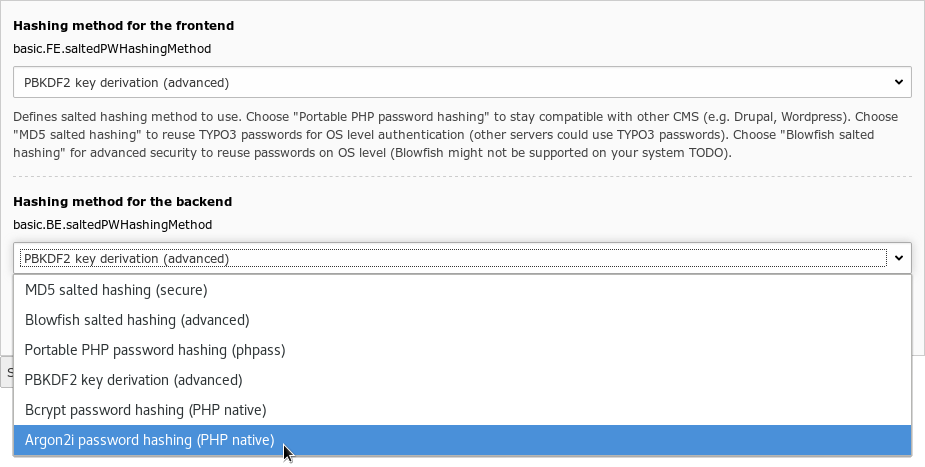
\includegraphics[width=0.65\linewidth]{Miscellaneous/SaltedPasswordsArgon2.png}
	\end{figure}

%	\begin{itemize}
%		\item Password hashes of existing users are automatically updated as required,
%			as soon as users log in
%	\end{itemize}

\end{frame}

% ------------------------------------------------------------------------------
% LTXE-SLIDE-START
% LTXE-SLIDE-UID:		2d8b3c8e-63ecbf7d-2a83935f-c111d446
% LTXE-SLIDE-TITLE:		Password Fields in the Install Tool
% LTXE-SLIDE-REFERENCE:	#81794 - Password fields in the Install tool
% ------------------------------------------------------------------------------

\begin{frame}[fragile]
	\frametitle{Varie}
	\framesubtitle{Install Tool Password Fields}

	\begin{itemize}
		\item L'Install Tool ora supporta il campo password per prevenire
			la visualizzazione di informazioni sensibili
	\end{itemize}

	\tabto{0.3cm}Ad esempio per il campo \texttt{Mail/transport\_smtp\_password}:

	\begin{figure}
		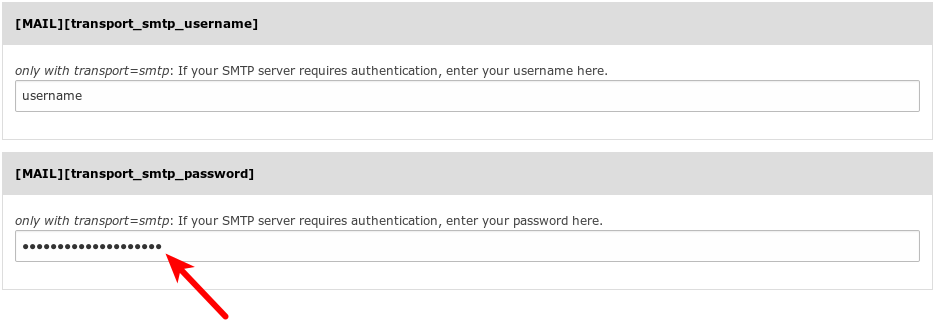
\includegraphics[width=0.95\linewidth]{Miscellaneous/InstallToolPasswordFields.png}
	\end{figure}

\end{frame}

% ------------------------------------------------------------------------------
